% CPSC 438 Final Project Paper
% Christopher Chute, David Brandfonbrener, Leo Shimonaka, Matthew Vasseur

% Author and Title Information
\newcommand*{\thetitle}{Wheels: An iOS Application for Yale's Special Services Van}
\newcommand*{\theauthor}{Christopher Chute}
\newcommand*{\duedate}{December 15, 2016}

% Document Settings
\documentclass[12pt, a4paper]{article}
\author{\theauthor}
\title{\thetitle}
\date{\duedate}
\usepackage[top=.75in, left=0.7in, right=0.7in, bottom=1.5in]{geometry}
\usepackage{amsmath, amsthm, amssymb}
\newtheorem{lem}{Lemma}
\usepackage{graphicx}
\usepackage{setspace}
\usepackage{enumitem}
\usepackage{booktabs}
\usepackage[T1]{fontenc}
\usepackage{titling}
\usepackage{hyperref}

% Multicolumn Formatting
\usepackage{multicol}
\setlength\columnsep{18pt}    % spacing between columns

\setlength{\droptitle}{-9em}
\posttitle{\par\end{center}\vspace{-.35em}}

% Header Formatting
\usepackage{fancyhdr}
\setlength{\headheight}{48pt}
\pagestyle{fancyplain}
%\lhead{\thetitle}
%\rhead{\theauthor\\\duedate}
%\rfoot{}
\cfoot{\thepage}
\graphicspath{{img/}}

\renewenvironment{abstract}
 {\small
  \begin{center}
  \bfseries \abstractname\vspace{-.5em}\vspace{0pt}
  \end{center}
  \list{}{%
    \setlength{\leftmargin}{0mm}% <---------- CHANGE HERE
    \setlength{\rightmargin}{\leftmargin}%
  }%
  \item\relax}
 {\endlist}

% ************************* End of Preamble ***********************
\begin{document}
\maketitle
\thispagestyle{empty}
\begin{abstract}
    This paper discusses the design and implementation of Wheels, an iOS application for hailing rides on Yale's Special Services Van. The app's objective is to replace its predecessor system for scheduling rides at Yale. In the previous system, users were required to call the Special Services dispatcher and provide the details (time, address, and accessibility requirements) for each ride. This system was inconvenient and had low bandwidth for scheduling rides. People often had to wait on hold for 5-10 minutes before reaching the dispatcher, and pickup locations were often miscommunicated. By contrast, Wheels eliminates waiting for the dispatcher (since many users can schedule rides simultaneously), and ride summaries are accompanied with GPS-based pickup information. The app allows users to quickly schedule rides and view their upcoming itinerary. Moreover, users can request to be picked up at their current GPS location. Wheels synchronizes through Amazon Web Services' (AWS) DynamoDB. All users' rides are stored in a DynamoDB table, and, using AWS Lambda triggers, the dispatcher receives notifications when a ride is scheduled, deleted, or needs to be executed. Users are authenticated using AWS Cognito, where NetIDs are checked against a whitelist maintained by Yale's Resource Office of Disabilities. This backend design was chosen to combine the extensibility of DynamoDB, security of Cognito, and the reliability of AWS in general. In short, Wheels replaces both the rider-dispatcher communication channel and the centralized data store for rides on Yale's Special Services Van. We hope that Wheels will improve the campus experience for all limited-mobility students, staff, and faculty at Yale.
\end{abstract}
\begin{multicols*}{2}
\section{Introduction}\label{sec:intro}
Wheels is an iOS application for scheduling rides on Yale's Special Services Van (``the Van''). The Van provides transportation to handicapped students and employees of Yale. That is, to be eligible to request rides with the Van, a student or employee needs to provide proof of a disability. Once cleared to ride, that person can request curbside transportation between any two points on Yale's campus. The Van operates on a 24-hour basis Monday-Friday, and between 6:00 PM and 7:30 AM on weekends. We note that ``the Van'' refers to the service itself rather than any particular vehicle. There are multiple vans and busses that are used to execute these rides, and they often operate simultaneously.

Prior to the development of Wheels, riders submitted requests by calling the dispatcher and reading the details of their ride over the phone. This system has a number of weaknesses. First, phone calls are relatively time-consuming. Second, phone lines are a lossy communication medium, and the dispatcher often misunderstands the NetID, pickup, or drop-off address of the rider. Third, phone calls to a single dispatcher cannot be parallelized. That is, the dispatcher can only talk to one rider at a time, so riders frequently need to wait on hold before they schedule a ride. This final point is an oft-encountered issue, and its importance is amplified by the existence of multiple Special Services Vans, which creates a mismatch in the capacity of the dispatcher and the drivers.

Wheels solves each of these problems by replacing the rider-dispatcher communication channel and the centralized data store for scheduling rides with the Van. On an iOS device, a rider schedules pickup with Wheels in one of two ways:
\begin{itemize}
	\item \textit{Schedule Ahead:} The rider completes two text fields denoting their pickup and drop-off location, selects their pickup time, and whether they need a wheelchair.
	\item \textit{On-Demand:} Using a map-based UI, the rider selects their pickup and drop-off locations. Pick-up location can be inferred from the rider's current GPS coordinates. The rider is prompted to select whether a wheelchair-accessible vehicle is needed, and the ride is requested immediately.
\end{itemize}
The ride information is sent to a central database, and forwarded to the dispatcher for execution. In each of these methods, the rider's NetID is automatically populated based on their login credentials.

We now describe how this solves the three problems posed earlier. First, requesting a ride with this mechanism takes roughly 30 seconds, much less time than an average phone call to the dispatcher. Second, this is a loss-less communication channel. The rider can view a summary of their ride that is exactly the same information seen by the dispatcher, so there is no room for miscommunication. Third, the database can support thousands of requests per second, so no rider will ever have to wait to schedule their ride. That is, requests are almost entirely parallelized and only limited by the database's write throughput.

In the sections that follow, we will describe the design decisions and implementation of Wheels. \hyperref[sec:user-interface]{Section \ref{sec:user-interface}} describes the user interface. In \hyperref[sec:local-db]{Section \ref{sec:local-db}}, we discuss the data model that locally backs the application. \hyperref[sec:back-end]{Section \ref{sec:back-end}} lays out the back end design of Wheels, including the centralized database and authentication mechanism. \hyperref[sec:takeaways]{Section \ref{sec:takeaways}} is perhaps the most relevant section for future seniors looking back on this project: This section explores the key lessons learned during the development of Wheels. In \hyperref[sec:future-plans]{Section \ref{sec:future-plans}}, we present the future plans for Wheels, especially regarding adoption by the Van. Finally, we conclude in \hyperref[sec:conclusion]{Section \ref{sec:conclusion}}.
\section{User Interface}\label{sec:user-interface}
The user interface of Wheels is heavily influenced by the iOS design principles published by Apple. In particular, the interface aims to be as minimal as possible while still providing the functionality necessary to schedule rides. There are four main pages: The login view, the Special Services information view, the on-demand request view, and the scheduled rides view.
\begin{center}
	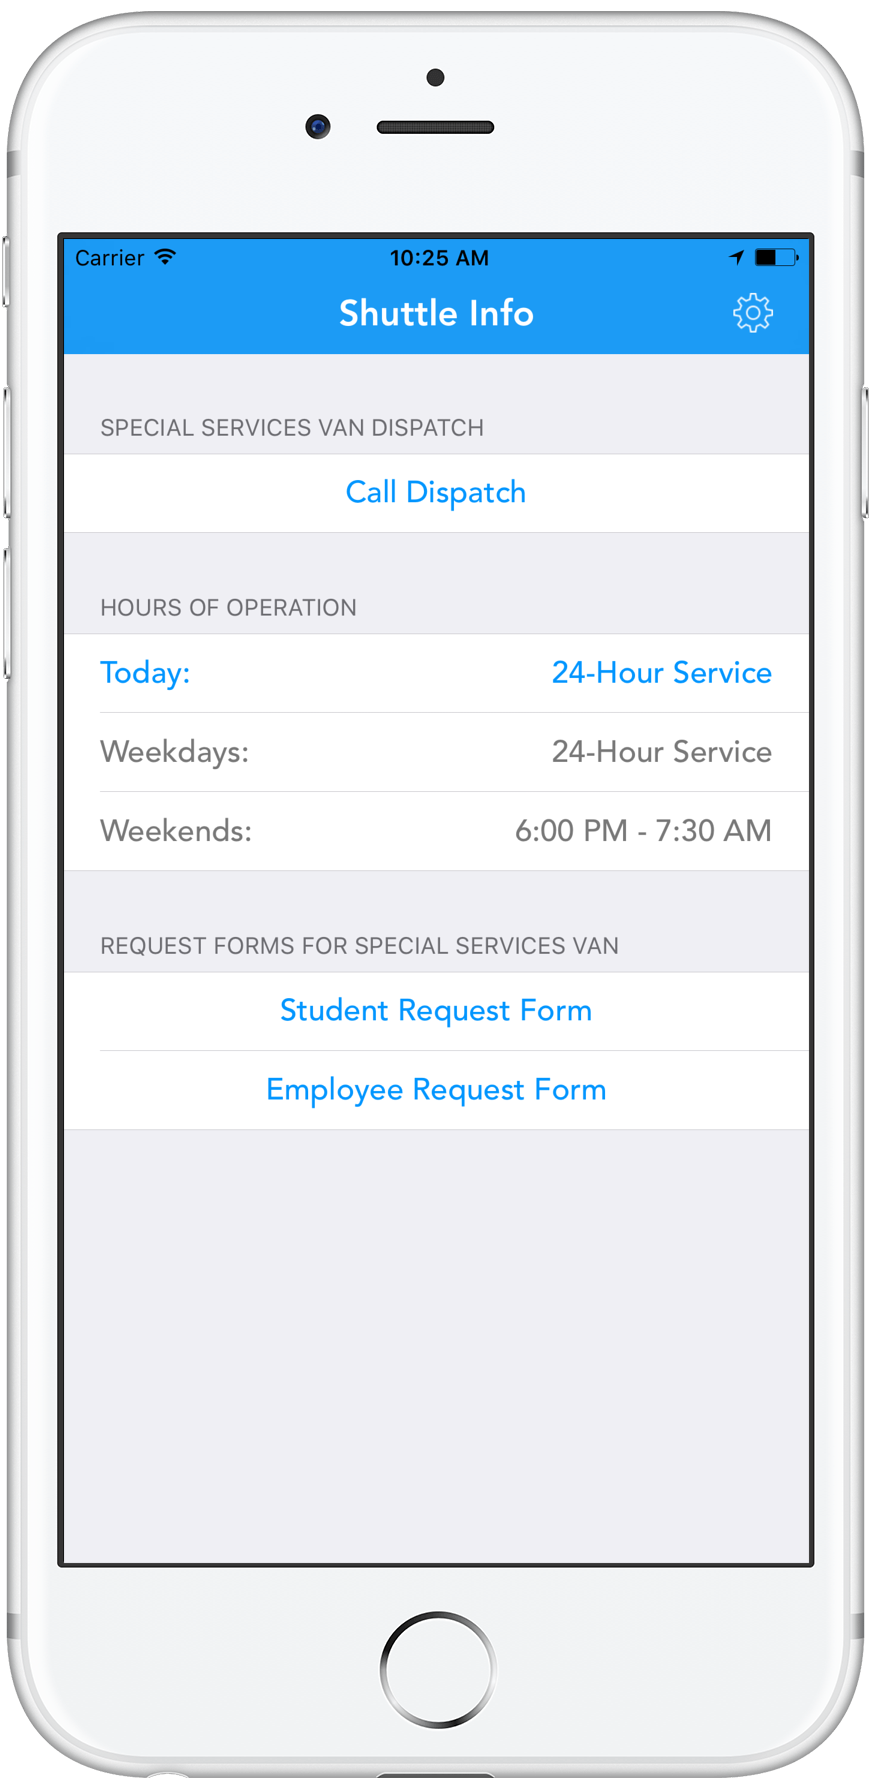
\includegraphics[keepaspectratio=true, width=0.30\textwidth]{screenshot-5.png}\\
	\textit{Figure 1: Special Services Information View.}
\end{center}

\subsection{Login and Information Views}
The login page receives the user's NetID and associated password. An animated login button guards access to the rest of the app. Once verified, the app is a 3-page array of screens arranged in horizontal sequence. The user simply swipes horizontally to move between the three pages.

The left-most of these three main pages is the Special Services information screen. This screen provides a button to call the Special Services hotline in case the user needs to speak directly to the dispatcher. The information screen also presents the Van's hours of service (updated given the day of the week). At the bottom of the information screen are links to the forms for requesting access to the Special Services Van. In the upper right-hand corner of the screen, there is a button for accessing the user's settings and logging out.

\subsection{On-Demand Request View}
The on-demand view is designed for requesting a ride for immediate execution. Since the driver will pick the rider up as soon as possible, an on-demand ride will commonly be requested to the user's current location. As such, the on-demand view is built around a street map that displays the user's current location. At the top of the view are two text fields for the pickup and drop-off addresses.
\begin{center}
	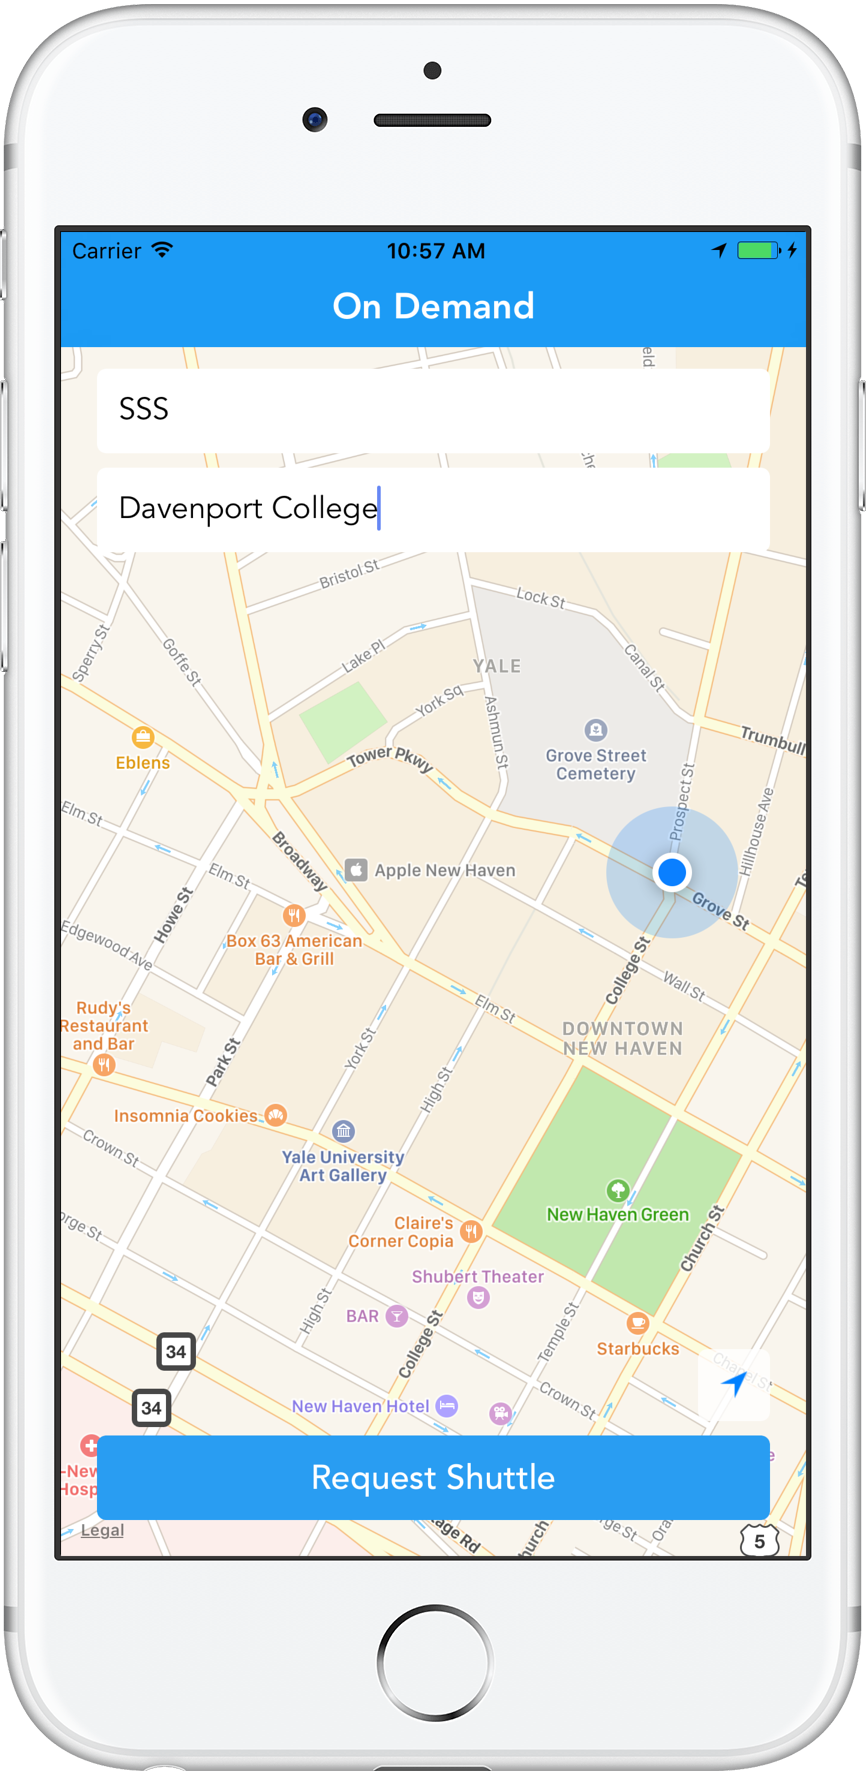
\includegraphics[keepaspectratio=true, width=0.35\textwidth]{screenshot-2.png}\\
	\textit{Figure 2: On-Demand Request View.}
\end{center}
If the user presses the ``current location'' symbol in the lower right-hand corner, the pickup address auto-completes to the user's current location. If the ``Request Ride'' button at the bottom of the screen is then pressed, the user's GPS coordinates will become the pickup address for the ride. Once the user has requested a ride, they will be prompted to select whether they need a wheelchair-accessible van. The ride is initially scheduled for five minutes from the request time, subject to update by the dispatcher.

\subsection{Scheduled Rides View}
\begin{center}
	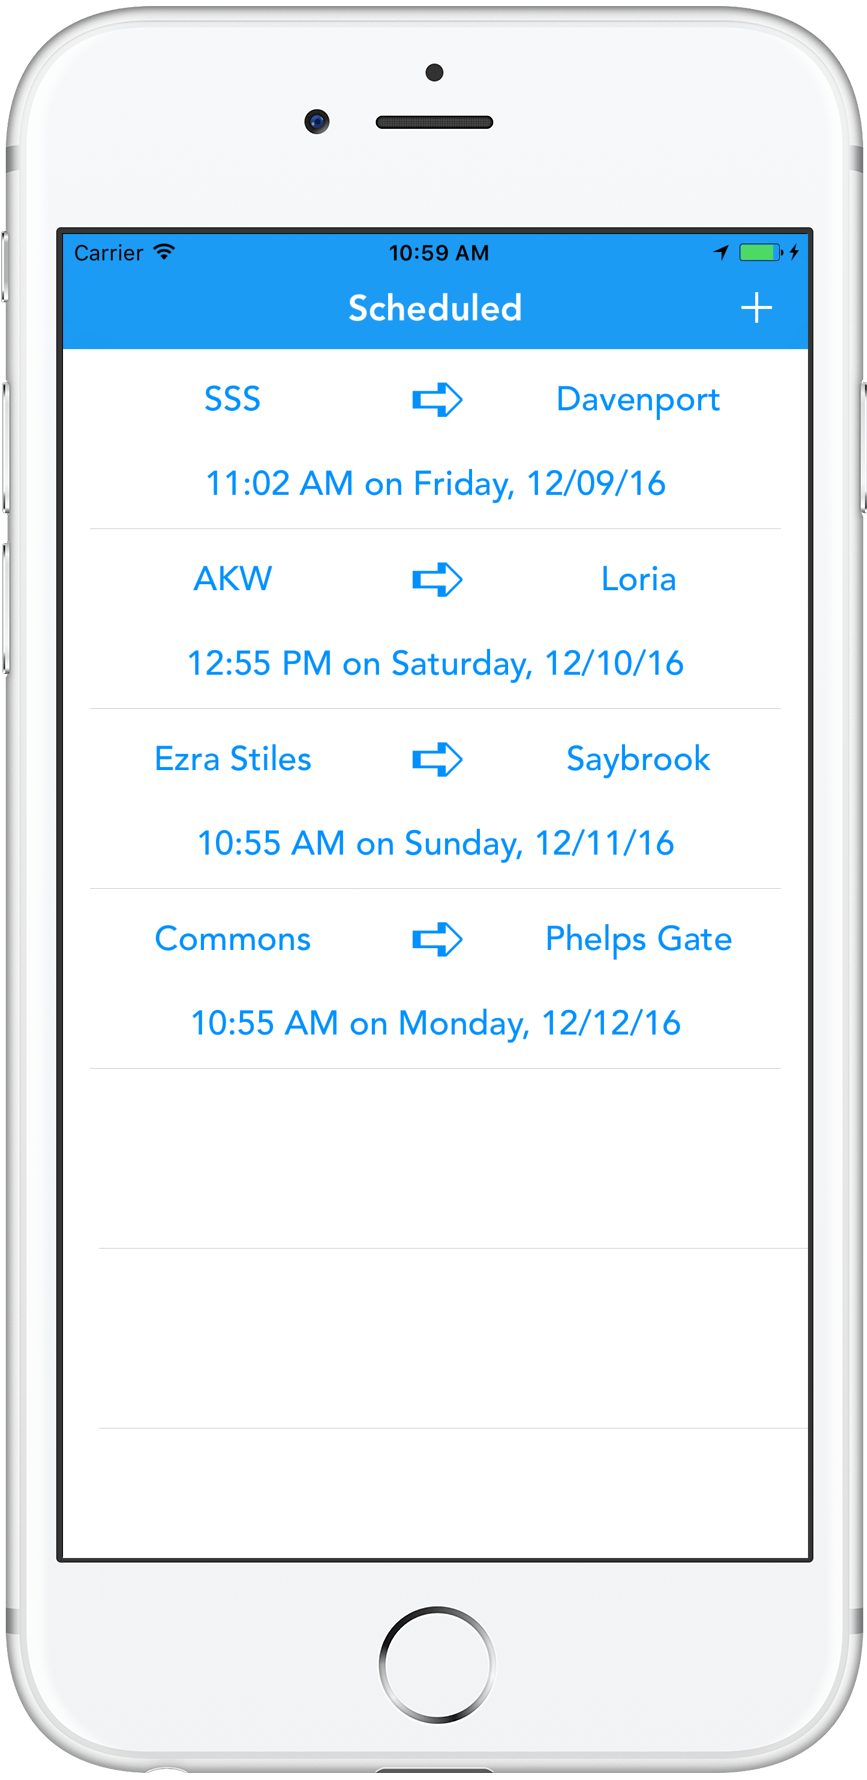
\includegraphics[width=0.35\textwidth]{screenshot-3.png}\\
	\textit{Figure 3: Scheduled Rides View.}
\end{center}
The scheduled rides view serves two functions. First, it displays all future rides scheduled by the current user. These rides are summarized in the rows of a table. Each row contains the pickup and drop-off addresses, as well as the scheduled pickup time of the ride. For example, the first row in Figure 3 (above) would be presented to summarize a ride from SSS to Davenport at the specified time. To reveal more information about the ride, the user simply taps on the row. This brings up another screen with the pickup address (GPS coordinates if applicable), drop-off address, scheduled time, and accessibility requirements of the ride.

Second, the scheduled ride view serves as the outlet for scheduling rides ahead of time. In the upper right-hand corner of the view, there is a $+$ symbol. By tapping the symbol, the user navigates to a new screen that receives input of the pickup location, drop-off location, date and time, and accessibility requirements of the ride. When the user taps ``Done'', the ride is submitted for approval by the dispatcher, and control is immediately returned to the user. A push notification shows up on the user's screen when their ride has been approved, and it automatically is slotted into the scheduled rides table.
\section{Local Data Store}\label{sec:local-db}
Wheels stores its information locally using Core Data, the object-oriented persistent storage solution provided by iOS. With Core Data, the developer constructs ``entities'', collections of attributes which are analogous to table schema. Once the attributes of an entity are defined, XCode will auto-generate a subclass of \texttt{NSManagedObject}, the parent class of all objects stored by Core Data. The resulting subclass can be constructed, manipulated, and destroyed in typical object-oriented fashion above the data tier. Importantly, each in-memory instance gets mapped to persistent storage when the programmer calls the \texttt{save} method on the associated \texttt{NSManagedObjectContext} instance. In this way, consistency is maintained between the persistent and in-memory data stores.

Wheels maintains two entities in its Core Data model: \texttt{ride}s and \texttt{rider}s. A \texttt{ride} has the string attributes \texttt{dateAndTime}, \texttt{fromAddress}, \texttt{toAddress}, and \texttt{guid}; and the boolean attribute \texttt{needsWheelchair}. Each ride has a relationship to a \texttt{rider}, where a \texttt{rider} has the attributes \texttt{netID}, \texttt{password}, and has a many-to-one relationship to a set of \texttt{ride}s called \texttt{scheduledRides}. With this model, all necessary information is stored about each ride, and all information for a given rider can be looked up efficiently.
\section{Back End Design}\label{sec:back-end}
The dispatcher must have a central database of all rides to effectively assign drivers to riders. Thus we needed to design a centralized backend. There are many IaaS offerings that would satisfy Wheels' modest requirements (CRUD, reasonable write throughput, and connection authentication). Of the candidates we considered, Amazon Web Services' (AWS) combination of DynamoDB, Cognito, and Lambda was deemed the most compelling package. Moreover, this package is offered at a very low price for the capacity required by Wheels.
\subsection{Remote Database: DynamoDB}
DynamoDB is a NoSQL database service offered by Amazon Web Services. Importantly for Wheels, the pricing model for DynamoDB is based on throughput rather than storage. This is favorable because the Van needs to maintain archives of provided rides, but has relatively low throughput requirements.

Wheels writes to a single DynamoDB table containing all user's rides. Each row includes the attributes of a \texttt{ride} as described in \hyperref[sec:local-db]{Section \ref{sec:local-db}}, in addition to the requesting rider's NetID. The DynamoDB table is configured to only accept requests from users authenticated through Cognito. The list of authorized NetIDs can be modified easily by the dispatcher, allowing the Disabilities Office to keep their list in sync with Wheels.
\subsection{Interfacing with the Dispatcher}
Whenever the DynamoDB table is modified (\textit{i.e.}, a row is added or removed), an AWS Lambda ``trigger'' is invoked. AWS Lambda is a service that will execute arbitrary code when a specific event occurs on another AWS service. Wheels takes advantage of this service by executing the code to notify the dispatcher whenever the DynamoDB table is modified. The details of how and when the dispatcher would prefer to receive notifications remain for future work.

\subsection{Authentication}
Another AWS offering, Cognito, handles the authentication requirements of Wheels. Cognito allows the developer to set up user pools, which are sets of credentials that can access your application. The dispatcher maintains a user pool of the NetIDs whitelisted by the Resource Office of Disabilities. Users can still download and login to Wheels without being on the whitelist, but they will be unable to request rides until their NetID is added. Finally, passwords with Cognito are independent of Yale CAS passwords.

\subsection{Example: A Typical Ride}
To illustrate how the sections of Wheels work in unison, we now step through a typical use case. Suppose that a user needs a ride from Sterling Chemistry Lab (SCL) to Davenport College at 3:00 PM today. The user first logs in to Wheels, providing their NetID and password. A request is sent to Cognito, and the result of that request is returned synchronously. Once in the app, the user swipes to the right-most screen, which is the scheduled rides view. When this view comes on screen, a request is sent to DynamoDB for all future rides scheduled by this user. The returned set of rides is used to populate the scheduled rides table. The user then clicks on the \texttt{+} symbol in the upper right-hand corner of the screen. The app segues to a form with text fields for the pickup address, drop-off address, pickup time, and accessibility requirements of the ride. When the user taps ``done'', the ride request is sent to DynamoDB (via an HTTP request generated by the AWS SDK). Upon arrival, the request is authenticated against the Cognito user pool. If approved, the request is then inserted as a row into the DynamoDB table, and a response is sent back to the user. An alert is displayed to notify the user once this response is received on the user's end.

This row insertion causes the registered AWS Lambda trigger to fire. The trigger generates a push notification that is received on the dispatcher's device. The dispatcher takes action by approving or rejecting the ride (\textit{e.g.}, if all vehicles will be busy, the dispatcher will reject the ride). This response updates the corresponding row in the DynamoDB table, and yet another Lambda trigger is invoked. This time, the student is notified of the dispatcher's decision to approve or deny the ride. If the ride was rejected, the student can request another ride or call the dispatcher to ask for alternative times. If the ride was approved, no further action is needed by the student.

When 2:45 PM rolls around (15 minutes before the pickup time), another AWS Lambda trigger fires to notify the dispatcher that the ride needs to be executed. This ensures that rides will not ``fall through the cracks,'' although typically this second notification will not be necessary. The dispatcher uses another system to make sure that rides are registered with the drivers when the ride is initially scheduled. This allows the drivers to plan ahead and communicate with the dispatcher if any problems arise. In any case, Wheels' gives up complete control of the ride once the dispatcher has been notified 15 minutes before execution. The dispatcher uses their previous mechanism to make sure the ride gets executed at 3:00 PM.

\section{Key Takeaways}\label{sec:takeaways}
We now share the major learning points encountered while developing Wheels. One obvious takeaway for the author was becoming familiar the iOS development platform tools (\textit{e.g.,} Swift, Cocoa Touch, XCode tools). However, these tools were not the focus of the project. The motivation to develop Wheels was to improve the Special Services Van experience, and iOS just happened to be the most popular mobile platform among Van users we surveyed. As such, we'll share more general principles that we learned while developing Wheels.

\subsection{User Interface Lessons}
When developing a user interface, we found that it's easy to have false illusions about your design. In particular, the design can become complicated and unintuitive without the developer realizing it. Moreover, because the design came out of the developer's head and thus fits their taste, everything looks appealing. To solve these problems, we found it helpful to expose the UI to as many people as possible during development stages. Those early viewers will catch many things that the developers missed. For instance, the first iteration of the login screen on Wheels was criticized heavily for its placement of text boxes and had to be remade.

The login screen issue could have been avoided in the first place by looking at popular examples on the App Store. As an inexperienced UI designer, the author found it helpful to look at the UI flows and standards of practice used by professional designers. For instance, almost all professional iOS apps have a login screen that positions the text boxes to be centered in the visible area above the keyboard. Although developers do not share their code, they must reveal their UI design by definition, so there are no excuses for not picking up on best practices.

The early viewers of Wheels had an instinctual feel for another good design principle: The most common use case should also be the easiest use case. That is, the UI should be designed so that the most common set of commands are the easiest to complete. For Wheels, this meant that the on-demand ride screen should be the default, and that it should be easy to request a ride to your current location. There were many other obvious applications of this principle, for instance that the user's NetID should be saved and automatically attached to the ride.

\subsection{Back End Principles}
The majority of development time for Wheels was spent architecting the data model and remote synchronization. Although this seems to be standard in mobile development, the extent of back end design time was probably exaggerated on this project. This is because the data model had to be augmented multiple times, and each time there were many steps to bring the app back online.

In this vein, we learned two major lessons when designing the data model for a mobile application. First, it is wise to plan the data model (including database schema, data structures, and data flow) in the earliest stages of development. The overhead to changing an application's data model is relatively high, so there is high incentive to get it right the first time. Moreover, the data model design will influence the design of layers above, including the presentation of data in the UI.

Second, there are many pre-made data tier solutions that should be taken advantage of, especially for the purpose of prototyping. For Wheels, Amazon Web Services proved to be very effective in accomplishing our goals at low (\textit{i.e.}, nearly zero) cost and low development time. Most of web services providers publish SDKs for major platforms, including iOS and Android. Aside from being fast and inexpensive to build on, these services provide security that would take years of developer time to match with an in-house solution.

\section{Future Plans}\label{sec:future-plans}
At the time of writing this paper, Wheels has not officially been adopted by the Special Services Van. Thus, while the actual development of Wheels is complete, there are a few steps to complete before the author's original goal of improving the Van experience is complete. These steps are as follows:
\begin{enumerate}[label=(\roman*)]
	\item \textit{ROD Whitelist NetID Authentication:} To give all current riders access to Wheels, we need to upload the official whitelist maintained by the Resource Office of Disabilities. The Cognito User Pool is already established for this task, but the actual NetIDs need to be added. Once in place, every person on the whitelist will receive a temporary password. Initially, only a subset of the whitelist will receive an invitation to download Wheels and try it for their next ride.
	\item \textit{Beta Testing:} The subset of Van riders who receives an invitation will be of a manageable size, so that the author can work with the dispatcher on streamlining the experience. We also imagine there will be some bugs revealed during this stage, which we will fix before officially rolling out the app.
	\item \textit{Driver-Side App:} Wheels focuses primarily on improving the experience for riders to schedule rides by replacing the rider-dispatcher communication channel. Additionally, there is room for improvement in the rider-driver and dispatcher-driver communication media. Eventually, we plan to provide a solution that is entirely integrated, so that the driver can see the same rider information as the dispatcher. This would also allow the rider to see the GPS location of the driver when the driver is approaching for pickup. Many other possibilities exist, such as optimally assigning the drivers to riders without the need for a dispatcher (more realistically, the dispatcher would be given suggestions).
	\item \textit{Available Times:} When a rider calls the dispatcher, they are frequently told that their original requested time is not available. This suggests that users of Wheels would frequently have their first request rejected by the dispatcher. To resolve this issue, we plan to implement a mechanism for riders to see what times have a shuttle available. One possible implementation would take an ``optimistic scheduling'' approach, where scheduling proceeds as usual, only prompting the user if there is a conflict. The dispatcher already needs to keep track of this information, so it would merely require moving their schedule to a database which can be accessed by Wheels users. For instance, if the Van is unavailable from now until 4:45 PM and I select 4:30 PM while scheduling my ride, an alert would pop up. The alert would say, ``The Van will be occupied at 4:30 PM. Does 4:45 PM work?'' or something to that effect. In essence, the user would be presented with the closest available time for pickup. This design would be consistent with the principle that the most common case (no conflict) should be the easiest case (schedule a ride normally) in the UI.
\end{enumerate}
This development of Wheels was motivated by the goal of improving the Special Services Van experience. This will not be completely accomplished until the Special Services Van is actually able to accept rides through Wheels. The initial implementation of Wheels is just one step toward accomplishing this goal, but the steps outlined above will carry it to completion.

\section{Conclusion}\label{sec:conclusion}
The Yale Special Services Van (``the Van'') serves the critical function of providing transportation to students, faculty, and staff with limited mobility. In researching this project, we found that most riders were satisfied with the Van but not with the scheduling mechanism. The predecessor system that Wheels aims to replace was flawed in many ways. By asking riders to place a phone call to the dispatcher every time they wanted a ride, the system wasted both riders' and drivers' time. The dispatcher's hotline was often busy, drivers were frequently directed to incorrect addresses, and recurring rides were difficult to request.

Wheels solves each of these problems in turn by providing an easy-to-use iOS interface for requesting rides. By all measurements, Wheels is faster and more reliable for scheduling rides with the Van. Users no longer need to wait on the phone until the dispatcher is available, since Wheels can handle hundreds of requests at a time. Moreover, Wheels adds new features to the Van, including the ability to request rides based on a user's GPS location. Users can view summaries of their upcoming rides, and easily cancel or request new rides. Just as phone-order retailers were replaced by stores which serve their customers via the Web, we believe that riders will heavily favor Wheels' iOS interface and Internet connectivity over phone-based requests.
\section{Acknowledgments}
We would like to thank Professor James Aspnes for serving as the advisor to this project. We would also like to thank the Resources Office of Disabilities for answering questions about the Van. Finally, we thank the riders who were surveyed during the first stages of the project, and those who have offered to test the application in the coming months.
\end{multicols*}
\end{document}

























